\documentclass[a4paper,12pt]{article}
\usepackage[left=2.5cm,right=2.5cm,top=2.5cm,bottom=2.5cm]{geometry} % Adjust page margins
\usepackage{xcolor,graphicx,framed}
\usepackage[normalem]{ulem}
\usepackage{amsmath}
\usepackage{gensymb}
%\usepackage{lastpage} % Required to print the total number of pages

\begin{document}

\newcommand{\HRule}{\rule{\linewidth}{0.4mm}} % Defines a new command for the horizontal lines, change thickness here

%----------------------------------------------------------------------------------------
%	HEADING SECTIONS
%----------------------------------------------------------------------------------------

\begin{minipage}{0.7\textwidth}
\begin{flushleft} 
\textsc{Universidad del Valle de Guatemala \\
Campus Central \\
Facultad de Ciencias y Humanidades \\
Departamento de Qu\'imica \\
Segundo ciclo, 2014 \\
Fisicoqu\'imica 1 \\
}
\end{flushleft}
\end{minipage}
~
\begin{minipage}{0.2\textwidth}
\begin{flushright}

\includegraphics[scale=0.3]{Logo_UVG} % Include a department/university logo
\end{flushright}
\end{minipage}\\

%----------------------------------------------------------------------------------------
%	TITLE SECTION
%----------------------------------------------------------------------------------------

\begin{center}
\HRule \\[0.4cm]
{ \bfseries Soluciones propuestas a los ejercicios en clase, 1}\\ % Title of your document
\HRule \\[0.4cm]
\end{center}

%----------------------------------------------------------------------------------------

\begin{enumerate}

 \item \textbf{\textit{(McQuarrie 16-4)} ?`A qu\'e temperatura las escalas de Celsius y Fahrenheit tienen el mismo valor num\'erico?} % Problema 2-4

Una forma de determinar esto, es encontrando la ecuaci\'on que relaciona estas dos escalas, lo cual puede hacerse a partir de los siguientes dos puntos coordenados:
\begin{center}
\begin{tabular}{c|c}
$\celsius$ & $^{\circ}\mathrm{F}$ \\\hline
0 & 32 \\
100 & 212
\end{tabular}
\end{center}

Como la relaci\'on es lineal, se puede obtener una ecuaci\'on de la forma $y=mx+b$ (usando $y$ para Fahrenheit y $x$ para Celsius), donde $m=\frac{\Delta y}{\Delta x}=\frac{212-32}{100-0}=\frac{9}{5}$ y $y(x=0)=m(0)+b=32\rightarrow b=32$. Las escalas tendr\'an el mismo valor n\'umerico cuando $x=y$, por lo que:
$$y=\frac{9}{5}y+32\rightarrow y=-40$$

 \item \textbf{\textit{(McQuarrie 16-6)} Las investigaciones en ciencia de superficies se llevan a cabo en c\'amaras de vacio ultra alto (ultra-high vacuum chambers) que pueden mantener presiones tan bajas como $10^{-12}$ torr. ?`Cu\'antas moleculas hay en un volumen de $1.00\;\mbox{cm}^{3}$ dentro de tal aparato a $298\;\mbox{K}$? ?`Cu\'al es el correspondiente volumen molar, $\bar{V}$, a esa presi\'on y temperatura?} % Problema 2-6

Para la primera pregunta:
$$PV=nRT\rightarrow n=\frac{PV}{RT}=\frac{(10^{-12}\;\mbox{torr})(1.00\;\mbox{cm}^{3})\left(\frac{1.00\;\mbox{dm}^{3}}{1000\;\mbox{cm}^{3}}\right)}{(62.364\;\mbox{dm}^3\cdot\mbox{torr}\cdot\mbox{K}^{-1}\cdot\mbox{mol}^{-1})(298\;\mbox{K})}=5.38\times 10^{-20}\;\mbox{mol}$$
Con lo que se puede determinar el n\'umero de mol\'eculas usando el n\'umero de Avogadro:
$$N=5.38\times 10^{-20}\;\mbox{mol}\left(\frac{6.022\times 10^{23}\;\mbox{mol\'eculas}}{1\;\mbox{mol}}\right)=3.24\times 10^{4}\;\mbox{mol\'eculas}$$
Para la segunda pregunta:
$$\bar{V}=\frac{V}{n}=\frac{1.00\;\mbox{cm}^{3}\left(\frac{1.00\;\mbox{dm}^{3}}{1000\;\mbox{cm}^{3}}\right)}{5.38\times 10^{-20}\;\mbox{mol}}=1.86\times 10^{16}\;\mbox{dm}^{3}\cdot\mbox{mol}^{-1}$$

 \item \textbf{\textit{(McQuarrie 16-11)} Se necesitan $0.3625\;\mbox{g}$ de Nitr\'ogeno para llenar un recipiente de vidrio a $298.2\;\mbox{K}$ y $0.0100\;\mbox{bar}$ de presi\'on. Si se necesitan $0.9175\;\mbox{g}$ de un gas diat\'omico homonuclear desconocido para llenar ese mismo recipiente bajo las mismas condiciones, ?`cu\'al es ese gas desconocido?} % Problema 2-11

Como se est\'a considerando comportamiento de un gas ideal y se tiene el mismo valor de $P$, $V$ y $T$, se tendr\'an en los dos gases la misma cantidad de $n$, que en el caso de Nitr\'ogeno, $N_2$, es:
$$n=\frac{0.3625\;\mbox{g}}{28.01\;\mbox{g}\cdot\mbox{mol}^{-1}}=1.295\times 10^{-2}\;\mbox{mol}$$
Por lo que el peso molecular del gas desconocido es:
$$M=m/n=(0.9175\;\mbox{g})/(1.295\times 10^{-2}\;\mbox{mol})=70.90\;\mbox{g}\cdot\mbox{mol}^{-1}$$
Como es un gas diat\'omico homonuclear, el peso mol\'ecular del \'atomo es la mitad ($70.90\;\mbox{g}\cdot\mbox{mol}^{-1}/2=35.45\;\mbox{g}\cdot\mbox{mol}^{-1}$), por lo que el gas desconocido es el gas Cloro.

 \item \textbf{\textit{(Atkins 1.6)} Un recipiente con volumen de $22.4\;\mbox{dm}^3$ contiene inicialmente $2.0\;\mbox{mol}$ de $H_2$ y $1.0\;\mbox{mol}$ de $N_2$, sumergido en un ba\~no t\'ermico a $273.15\;\mbox{K}$. Todo el $H_2$ reacciona con suficiente $N_2$ para formar $NH_3$. Calcular las presiones parciales y la presi\'on total de la mezcla final.} % Problema 1.6 de Atkins

La ecuaci\'on de la reacci\'on es la siguiente:
$$3H_2(g)+N_2(g)\rightarrow 2NH_3(g)$$
Como todo el $H_2$ reacciona, podemos calcular la cantidad de los otros dos gases presentes:
$$n_{N_2}=1.0\;\mbox{mol}-2.0\;\mbox{mol de H}_2\left(\frac{1\;\mbox{mol de N}_2}{3\;\mbox{mol de H}_2}\right)=\frac{1}{3}\;\mbox{mol}$$
$$n_{NH_3}=2.0\;\mbox{mol de H}_2\left(\frac{2\;\mbox{mol de NH}_3}{3\;\mbox{mol de H}_2}\right)=\frac{4}{3}\;\mbox{mol}$$
Lo que da $n_T=n_{H_2}+n_{N_2}+n_{NH_3}=0+1/3+4/3=5/3\;\mbox{mol}$, que podemos usar para determinar la presi\'on total:
$$P=\frac{nRT}{V}=\frac{(5/3\;\mbox{mol})(8.314\times 10^{-2}\;\mbox{dm}^3\cdot\mbox{bar}\cdot\mbox{K}^{-1}\cdot\mbox{mol}^{-1})(273.15\;\mbox{K})}{22.4\;\mbox{dm}^3}=1.69\;\mbox{bar}$$
$$x_{H_2}=\frac{n_{H_2}}{n_T}=0\rightarrow P_{H_2}=0$$
Calculando las fracciones molares, las preciones parciales ser\'ian:
$$x_{N_2}=\frac{n_{H_2}}{n_T}=\frac{1/3}{5/3}=1/5\rightarrow P_{H_2}=x_{H_2}P_T=(1/5)(1.69\;\mbox{bar})=0.338\;\mbox{bar}$$
$$x_{NH_3}=\frac{n_{NH_3}}{n_T}=\frac{4/3}{5/3}=4/5\rightarrow P_{NH_3}=x_{NH_3}P_T=(4/5)(1.69\;\mbox{bar})=1.35\;\mbox{bar}$$

\newpage

 \item \textbf{\textit{(McQuarrie 16-7)} Usar la siguiente informaci\'on de un gas desconocido a $300\;\mbox{K}$ para determinar la masa molecular del gas.} % Problema 2-7

\begin{center}
\begin{tabular}{c|c c c c c}
$P/bar$ & 0.1000 & 0.5000 & 1.000 & 1.01325 & 2.000 \\\hline
$\rho/g\cdot L^{-1}$ & 0.1771 & 0.8909 & 1.796 & 1.820 & 3.652 
\end{tabular}
\end{center}

De primero, determinemos la relaci\'on entre la presi\'on y la densidad. Considerando un gas ideal y que $n=m/M$, donde $M$ es la masa molecular del gas y usando $\rho=\frac{m}{V}$:
$$PV=nRT\rightarrow \frac{P}{RT}=\frac{m}{VM}\rightarrow P=\frac{RT}{M}\rho$$
Lo que indica que una gr\'afica de $P$ vs. $\rho$ nos deber\'ia de dar una relaci\'on lineal, para la cual la pendiente viene dada por $RT/M$. La grafica de los datos con su regresi\'on lineal es la siguiente:
\begin{center}
 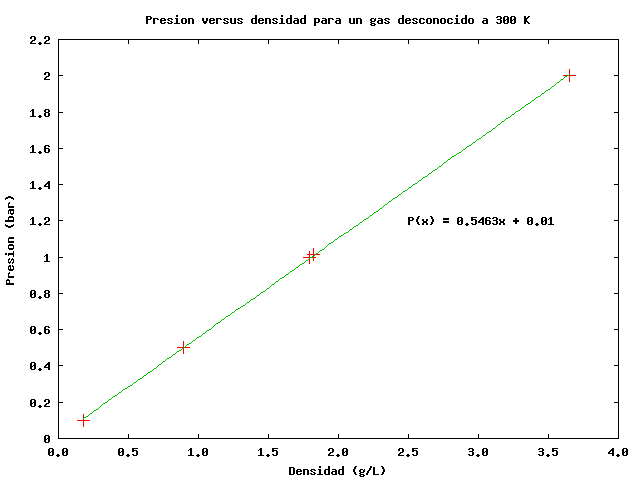
\includegraphics[scale=0.9]{figure1}
\end{center}
Por lo que: 
$$\frac{RT}{M}=0.5463\;\mbox{bar}\cdot\mbox{L}\cdot\mbox{g}^{-1}\rightarrow M=\frac{(8.314\times 10^{-2}\;\mbox{L}\cdot\mbox{bar}\cdot\mbox{K}^{-1}\cdot{mol}^{-1})(300\;\mbox{K})}{0.5463\;\mbox{bar}\cdot\mbox{L}\cdot\mbox{g}^{-1}}$$
Con lo que se obtiene que el gas desconocido tiene una masa molecular de $45.66\;\mbox{g}\cdot\mbox{mol}^{-1}$.

\end{enumerate}
 
\end{document}
